%----------------------------------------------------------------------------------------
% Ajedrez
%----------------------------------------------------------------------------------------

Este proyecto consiste en programar un jugador de ajedrez haciendo uso de las técncias de IA clásica.

\section{Meta}

El alumno implementará un agente inteligente capaz de jugar ajedrez contra un ser humano.

\section{Objetivos}

Que el alumno(a):
\begin{compactitem}
 \item Implemente un agente inteligente para un juego.
 \item Implemente un algoritmo de búsqueda con adversarios aplicándolo en un escenario real, transfiriendo sus conocimientos sobre \emph{acciones}, \emph{acciones aplicables}, \emph{estados} y \emph{nodos búsqueda}.
 \item Diseñe su propia estructura para implementar el algoritmo.
 \item Utilice un función heurística para truncar la profundidad a la que trabajará el algoritmo.
\end{compactitem}


\begin{auxcode}
 \caption{Ajedrez}
 \centering
 \hurl{\auxprefix ia-ajedrez}
\end{auxcode}


\section{Introducción}

El juego del Ajedrez es un ejemplo excelente de problema de planeación sobre un espacio de estados discreto que se puede resolver mediante búsqueda.  El espacio de estados corresponde a todos los posibles tableros del juego: todas las posibles combinaciones de posiciones de figuras en él más aquellas que pudieran haber sido capturadas [\fref{fig:tableroAjedrez}].  El espacio es enorme, sin embargo, el problema se puede enfrentar tan sólo con técnicas clásicas.  La fecha 11 de mayo de 1997 quedó marcada como el día en que la IA DeepBlue derrotó al campeón humano de ajedrez Garry Kasparov\footnote{\hurl{https://ethic.es/2024/03/el-dia-que-kasparov-perdio-contra-deep-blue/}}.  DeepBlue utilizó búsqueda sobre el espacio de estados, haciendo evaluaciones de los estados mediante una función heurística.  En otras palabras: en este curso ya estudiaste todo lo necesario para comprender e incluso implementar un sistema igual.  Para este proyecto harás una implementación un poco más sencilla pero sólo por cuestiones de tiempo.

\begin{figure}
 \centering
 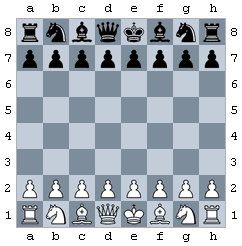
\includegraphics[width=0.5\textwidth]{ajedrez/tableroAjedrez}
 \caption{Estado inicial para el problema de jugar al ajedrez.}
 \label{fig:tableroAjedrez}
\end{figure}

Las reglas del juego son mundialmente conocidas, un sitio donde puedes encontrar todos los detalles es \hurl{https://help.gnome.org/users/gnome-chess/stable/index.html.es}.  Las reglas más importantes son:
\begin{itemize}
 \item La \fref{fig:tableroAjedrez} describe el estado inicial.
 \item Las piezas sólo pueden moverse a casillas desocupadas, a menos que puedan realizar la captura del pieza contraria.
 \item Los peones sólo pueden moverse una casilla hacia adelante, pero capturan movéndose en diagonal hacia el frente un cuadro.
 \item Las torres se desplazan horizontal y verticalmente.
 \item Los alfiles se desplazan diagonalmente.
 \item La reina puede moverse horizontal, vertical y diagonalmente.
 \item El puede moverse a cualquiera de las ocho casillas a su alrededor.
 \item Torres, alfiles y reina pueden desplazarse tantas casillas como quieran en sus direcciones válidas, siempre que no se topen con otra pieza.  Si la otra pieza es enemiga la pueden capturar y quedarás colocados en el lugar que ocupaba la otra pieza.
 \item Los caballos son los únicos que pueden saltar y su desplazamiento es en forma de L: dos cuadros verticalmente y uno horizontal ó dos horizonales y uno vertical, en la dirección que prefiera.  Sólo captura a la pieza que se encuentre en su casilla final.
 \item Se dice que el rey está en \code{jaque} si una pieza enemiga se coloca donde lo puede capturar y el jugador tiene la obligación de rescatar a su rey.
 \item El juego termina cuando uno de los jugadores logra capturar al rey del otro.  Cuando un rey se encuentra en posición de jaque, sin que éste tenga escapatoria posible el juego termina (\emph{jaque mate}).
\end{itemize}



\section{Desarrollo e implementación}

Para este proyecto programarás a un agente inteligente para jugar ajedrez contra él.  Para ello en este paquete se te entrega un proyecto \code{JavaFX} con la interfaz gráfica para mostrar un ajedrez [\fref{fig:ajedrezfx}].

\begin{figure}
 \centering
 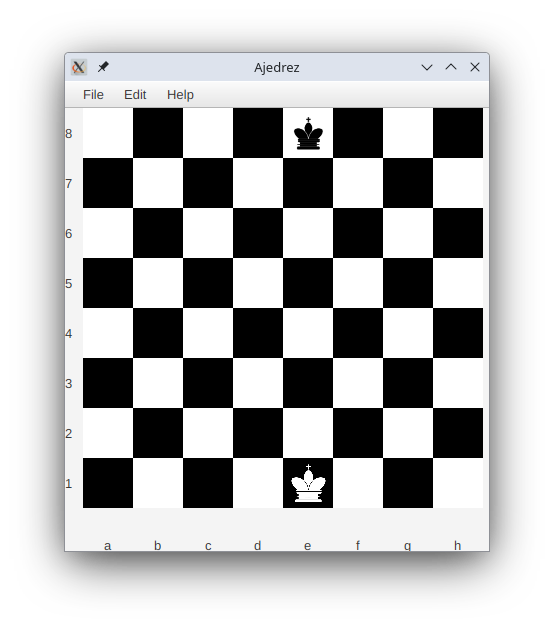
\includegraphics[width=0.5\textwidth]{ajedrez/ajedrezfx}
 \caption{Interfaz gráfica en \code{JavaFX} para programar el juego de ajedrez.}
 \label{fig:ajedrezfx}
\end{figure}

\subsection{Tareas a realizar}

Las tareas que debes realizar son las siguientes.  Incluye pruebas unitarias que muestren que cada parte de tu código funciona correctamente.

\begin{enumerate}
\subsubsection{Parte I: Reglas del ajedrez}
 \item Completa el proyecto que se te entrega.  El paquete:
\begin{center}
 \code{ia.ajedrez.modelo}
\end{center}
  ya incluye las clases para representar a las piezas del juego y sus movimientos legales, excepto por la \textbf{torre} y el \textbf{alfil}.  Agrega estas clases faltantes.

 \item En la clase \code{Juego} completa el método \code{jugadaEsVálida}, aquí deberás tomar en cuenta ya las posiciones de todas las piezas en el tablero.  Observa que hay varios tipos de jugadas: movimiento, captura, enroque corto y enroque largo. Los caballos pueden saltar pero las otras piezas no.

 Añade métodos o lo que encuentres necesario.  Recuerda que es tu proyecto.  Observa que este paso corresponde a determinar si una acción es aplicable en un estado dado.

 \item Completa el constructor por defecto de \code{Tablero} colocando todas las piezas en el estado inicial.  Para ello deberás también agregar imágenes para las piezas del tablero, el programa las escala así que no tienes que preocuparte demasiado por la escala, puedes descargar las imágenes de internet o usar grafos de fuentes.  Agrega las imágenes completando el método
 \begin{center}
  \code{private void creaVistasDePiezas()}
 \end{center}
 de la clase \code{vistas.VistaTablero}.


 \item Completa ahora el método \code{ejecutaJugada} en la misma clase para que los cambios sugeridos por la jugada se vean reflejados en el tablero.  Recuerda almacenar qué jugada fue la que produjo el cambio en el tablero.  En la segunda parte del proyecto este historial corresponderá a las \emph{acciones aplicadas}.  Así que observa bien cómo haces tu diseño, pensando en resolver la segunda parte.

 \item Regresa ahora a la clase \code{Tablero} y completa \code{hayJaqueMate}.

 \item Finalmente prepara tu heurística: completa el método \code{calificación} de la clase \code{Tablero}.  Como no será posible explorar todo el espacio de estados del ajedrez, habrá que truncar el algoritmo de búsqueda con adversarios que implementarás.  Para ello, lo que harás es otorgar una calificación a cualquier tablero, para determinar \textit{quién va ganado la partida}.

 Usa una función que pondere los valores siguientes:
 \begin{enumerate}
  \item Valores: suma puntos según el valor de cada pieza blanca en el tablero y réstalos por cada pieza negra.

  \item Dominio del tablero:  Por cada pieza, suma un punto por cada escaque libre al que pueda moverse dicha pieza si es blanca y resta un punto si la pieza es negra.
 \end{enumerate}

 Devuelve un valor entero.  Si uno de los jugadores está en jaque mate, devuelve el entero más grande si ganaron las bancas o el entero más pequeño si ganaron las negras.
       
\subsubsection{Parte II}

 \item Crearás ahora a un agente para que mueva a las piezas negras.  Modifica a la clase juego para que, cada vez que el turno pase a mano de las negras, se mande llamar una función que elija cómo mover la pieza y, una vez movida, regrese el turno a las blancas.

 \item Para explorar el espacio de estados puede ser necesario crear copias de un estado y modificarlas en puntos estratégicos de la búsqueda.  Completa el constructor copia de la clase \code{Tablero}.  Para esto, dado que las piezas almacenan su posición, también deberás crear constructores copia para poder clonar las piezas en el tablero.

 \item Implementa el algoritmo Min-max en su versión recursiva, de modo que vaya realizando una búsqueda en profundidad sobre el espacio de tableros.  La mejor forma de aprovechar la memoria es no crear tantas copias del tablero, sino utilizar los objetos tipo \code{Jugada} para revertir las modificaciones al tablero cuando la recursividad deba regresar a un nodo búsqueda anterior.  Crea copias únicamente cuando lo requieras para no perder información importante.

 Deberás definir una profundidad límite la cual tratarás como si fuera el fin del juego, aquí utilizarás la función \code{calificación} para asignar el puntaje al tablero.

 Mide cuál es la profundidad máxima que puede alcanzar tu algoritmo sin dejar esperando demasiado al jugador blanco.

 \textbf{Nota:} No olvides incluir pruebas unitarias que muestren que cada parte de tu modelo funciona.

 \item Se otorgará un punto extra a quien sustituya Min-max por poda alfa-beta.

 \item Los empates son más complejos de detectar, por lo que su implementación se dejará para obtener otro punto extra si implementas este caso completo o décimas si sólo implementas algunos casos.  Se dice que el juego queda \emph{tablas} por varios motivos \footnote{\hurl{https://help.gnome.org/users/gnome-chess/stable/chess-rules.html.es}}:
 \begin{description}
  \item [Por acuerdo]  Ambos jugadores se rinden... pero tu PC no se rinde, así que no aplicaremos esta regla.
  \item [Rey ahogado]  El jugador que tiene que mover no tiene movimientos legales y su rey no está en jaque.
  \item [*Repetición triple] La misma posición sucede tres veces con el mismo jugador y si cada jugador tiene el mismo conjunto de movimientos legales las tres veces, incluyendo comer y enroque.
  \item [Regla de los cincuenta movimientos] Después de 50 movimientos de cada jugador no se ha movido o capturado un peón.
  \item [Jaque mate imposible] Todos los peones se han capturado y un jugador sólo tiene su rey, mientras que el otro jugador también tiene solamente su rey o su rey y un caballo o un alfil.
 \end{description}

\end{enumerate}


\section{Requisitos y resultados}

Básicamente, deberás entregar un ajedrez que se pueda jugar.  El agente manejado por la PC usará Min-max para elegir su tirada.  Juega algunas partidas y asegúrate de que puedes iniciar bien la partida, jugar contra la computadora y que se declara al ganador correctamente cuando ocurre y jaque mate.  Edita tu \code{README.md} con las instrucciones adecuadas para que cualquier usuario pueda ejecutar tu aplicación.
